%Author Callum Davidson, C3347372, Software Engineering COMP1010
%The report will contain a brief review of research works in a Knowledge Area of interest
%(including a short literature review). The report will look at works at the intersection of the
%Knowledge Area and a chosen topic
% This report needs to be 10 pages long and is due Monday week 7 at 0800, 
% Font needs to be time new roman, single spaced with margins that should not exceed 1cm 
%The 10 pages length does not include references
%No more than 4 small figures/tables are aloud 

% Ideas
%1: Predicitve models for marketing campaigns based on text and recurrent neural networks https://www.sciencedirect.com/science/article/abs/pii/S0957417422016360?via%3Dihub
% https://www.mdpi.com/1999-5903/11/1/5  Forecasting E-Commerce Products Prices by Combining an Autoregressive Integrated Moving Average (ARIMA) Model and Google Trends Data
%2 Click through rate model of ecommerce https://www.sciencedirect.com/science/article/abs/pii/S0957417422011459?via%3Dihub
% Databases for finding information Web of Science (https://www.webofknowledge.com/).
%DBLP The Computer Science Bibliography (https://dblp.uni-trier.de/).
%3 Enhancing e-cmmerce using pretrained language model https://arxiv.org/abs/2302.04443
%4 Algorithms to live by , Explore exploit algorithm A/B testing, amazon caching "anticipatory package shipping. 
%5 Simulated annealing for influence maximization problem of online social networks, how to market to the most amount of people. https://www.sciencedirect.com/science/article/pii/S1877050917317167?via%3Dihub
%6 Predictive model of consumer onine purchase behaviour based on data mining https://www.inderscience.com/offer.php?id=128405
%7 Consumer fraud in online shopping, detecting risk indicators through data mining https://www.tandfonline.com/doi/abs/10.1080/10864415.2022.2076199?journalCode=mjec20
%8 Cluster Analysis e commerce https://www.inderscienceonline.com/doi/abs/10.1504/IJWBC.2023.128409
%9 Precise marketing data mining method of E-commerce platform based on association rules https://link.springer.com/article/10.1007/s11036-021-01886-3
%A Novel Approach of Product Recommendation Using Utility-Based Association Rules https://www.igi-global.com/gateway/article/289574

%10 https://link.springer.com/chapter/10.1007/978-3-031-06794-5_30 Research on E-commerce Customer Churn Based on RFM Model and Naive Bayes Algorithm

% A deep mining method for consumer behaviour data of e-commerce users based on clustering and deep learning https://www.inderscience.com/offer.php?id=128410
% https://scholarspace.manoa.hawaii.edu/items/c9f8d5d4-4dae-4a95-8598-967c0911adcd Let me Entertain You – the Influence of Augmented Reality on Purchasing Intention in E-Commerce
%https://arxiv.org/abs/2203.10996 Technologies for AI-Driven Fashion Social Networking Service with E-Commerce

\documentclass{article}

\title {This is a title}

\author {Callum Davidson}

\date{\today}
\usepackage{graphicx}
\usepackage{amsmath}


\begin{document}
\maketitle
\tableofcontents


\begin{abstract}
Abstract goes here
\end{abstract}

\section{Introduction}
This is an introduction
\label{sec:intro}

\section{Predicitve model marketing camplaign}
This article presents a mofel for predicting trends in marketing campaign influence  in e-commerce, or as defined in the paper " The extent to which a marketing campaign is spread among the user groups on that e-commerce platform". 

\subsection{More about something}

\subsection{Even more about something}

\section{Click through rate model based on user interest and temporal behaviour }


CLick through rate is the ratio of the number users who click on an ad to the number of users who viewed the ad https://en.wikipedia.org/wiki/Click-through_rate
paper designs a structure of time-weighted gated recurrent units (TW-GRU) to predict users’
short-term interest and long-term interest. 
The paper found that when anlayzing user behviour data that in shorter time intervals, the item's a user purchased were in related categories whereas in longer term patterns the users purchased items were found to be less relevant to eachother. 
\subsection{Game Theory}
\subsection{AIMD}
\subsection{optimal stopping}
\subsection{Scheduling}
\subsection{explore/exploit}

\section{Product Life Cycle} 

In section \ref{sec:intro}, we \ldots




\begin{figure}
\centering
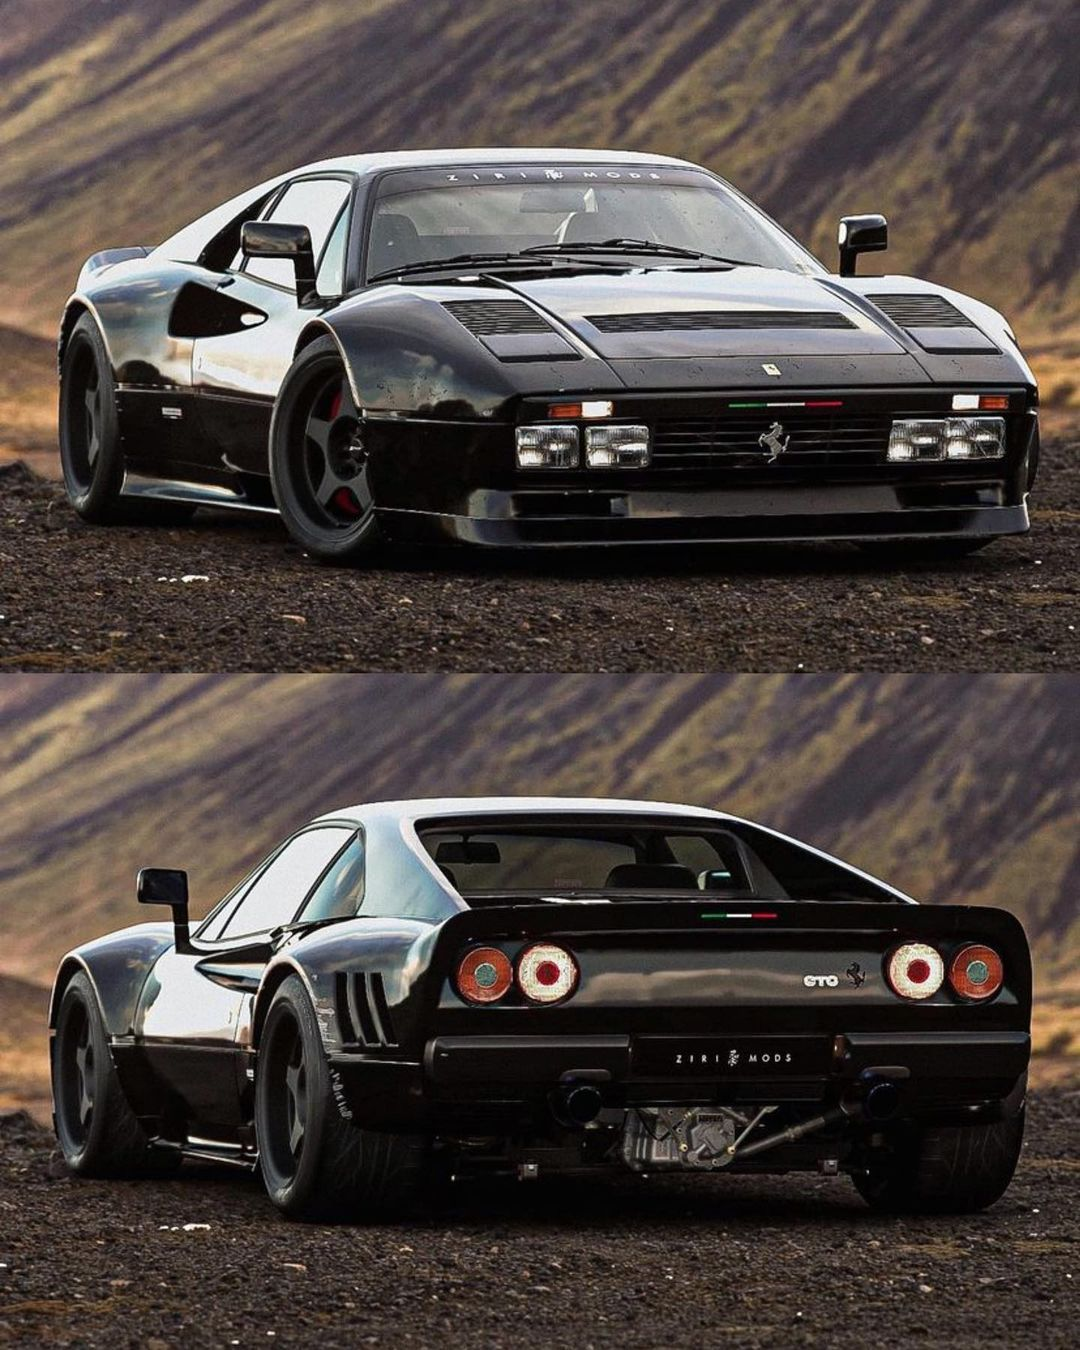
\includegraphics[ width=1.2\textwidth] {Ferrari288GTO.jpg}
\caption{\label{fig:Ferrari288GTO} Ferrari 288 GTO }
\end{figure} 


\begin {enumerate}
\item Topic idea : 
\item Topic idea : 
\end {enumerate}




\begin{equation}
\label {eq:something} 
\min_{x,y} { (1-x)^2 + 100(y-x^2)^2}\\
\end{equation} 

\begin{equation*} % * is without enumeration
\beta_i = 
\frac{\operatorname{Cov} (R_i, R-m)}
	{\operatorname{Var} (R_m)}
\end{equation*} 
In \eqref{eq:something}, we have \ldots


\begin{align*}
(x+1)^3 &= (x+1)(x+1)(x+1) \\
&= (x+1)(x^2 + 2x + 1) \\
&= x^3 + 3x^2 + 3x + 1
\end{align*}

Let X{1}, X{2},...,Xn be a sequence of independant and identically distrubuted random variables with E[X{i}] and 
\begin{equation*}
S{n}=
\frac{1}
	{n}
\sum_{i=1}^{n} X{i}
\end{equation*}


\section {Price}

\begin{tabular}{|l|r|r|} \hline% Argument column specifies column alignment
Item                       & Qty      &     MSRP \$ \\\hline
Ferrari 288 GTO      & 1         &      5     \\\hline

Lamborghini Miura   &2          &      3      \\

Porche 911 GT3       &3          &      2.5    \\\hline
\end{tabular}
\cite{Brooks1997Methodology}
shows that \ldots. Clearly,
all odd numbers are prime


Conclusion goes here


Acknolwdgement goes here

\bibliography{TestReferences}
\bibliographystyle{unsrt}

\end{document}

%Up to typesetting excersise 2